\documentclass{beamer}

\usefonttheme{professionalfonts} % using non standard fonts for beamer
\usefonttheme{serif} % default family is serif

\usepackage{hyperref}

\usepackage{animate}

\usepackage{graphicx}

\def\Put(#1,#2)#3{\leavevmode\makebox(0,0){\put(#1,#2){#3}}}

\usepackage{color}

\usepackage{tikz}

\usepackage{amssymb}

\usepackage{enumerate}

\usepackage{pdfpages}

% \usepackage{minted}

\newcommand\blfootnote[1]{%

  \begingroup

  \renewcommand\thefootnote{}\footnote{#1}%

  \addtocounter{footnote}{-1}%

  \endgroup

}

\makeatletter

%%%%%%%%%%%%%%%%%%%%%%%%%%%%%% Textclass specific LaTeX commands.

 % this default might be overridden by plain title style

 \newcommand\makebeamertitle{\frame{\maketitle}}%

 % (ERT) argument for the TOC

 \AtBeginDocument{%

   \let\origtableofcontents=\tableofcontents

   \def\tableofcontents{\@ifnextchar[{\origtableofcontents}{\gobbletableofcontents}}

   \def\gobbletableofcontents#1{\origtableofcontents}

 }

%%%%%%%%%%%%%%%%%%%%%%%%%%%%%% User specified LaTeX commands.

\usetheme{Malmoe}

% or ...

\useoutertheme{infolines}

\addtobeamertemplate{headline}{}{\vskip2pt}

\setbeamertemplate{theorems}[numbered]

\setbeamercovered{transparent}

% or whatever (possibly just delete it)

\makeatother

\begin{document}
\title[Discussion 7]{CS/MATH 111, Discrete Structures - Fall 2018. \\ Discussion 7 - Non-homogeneous Recurrences,  Tiling \& Red Riding Hood problem }
\author[CS111]{Andres, Sara, Elena}
\institute[Fall'18]{University of California, Riverside}
\makebeamertitle
\newif\iflattersubsect

\AtBeginSection[] {
    \begin{frame}<beamer>
    \frametitle{Outline} 
    \tableofcontents[currentsection]  
    \end{frame}
    \lattersubsectfalse
}

\AtBeginSubsection[] {
    \begin{frame}<beamer>
    \frametitle{Outline} 
    \tableofcontents[currentsubsection]  
    \end{frame}
}

\section{Non-homogeneous recurrence}

\begin{frame}{Non-homogeneous recurrence\footnote{\scriptsize Proof available at [Rosen, 2015. pg 521].}}
    \begin{theorem}\label{theo:1}
    {\Large $$f_n = f_n^{'} + f_n^{''}$$}
    
    If $\{f_n^{''}\}$ is a particular solution of the non-homogeneous linear recurrence relation with constant coefficients: 
    $$ f_n = c_1 \cdot f_{n-1} + c_2 \cdot f_{n-2} + \cdots + c_k \cdot f_{n-k} + g(n) $$
    then every solution is of the form $\{f_n^{'} + f_n^{''}\}$, where $\{f_n^{'}\}$ is a solution of the associated homogeneous recurrence relation.
    \end{theorem}
\end{frame}

\begin{frame}{Non-homogeneous recurrence}
    Solve next non-homogeneous recurrence with initial condition $f_0=0$, $f_1=2$ and $f_2=7$:
    \begin{equation}\tag{1}
        f_n = 6 \cdot f_{n-2} + 4 \cdot f_{n-3} + 2^n
    \end{equation}
\end{frame}

\begin{frame}{Non-homogeneous recurrence}

    {\small Solve next non-homogeneous recurrence with initial condition $f_0=0$, $f_1=2$ and $f_2=7$:
    \begin{equation}\tag{1}
        f_n = 6 \cdot f_{n-2} + 4 \cdot f_{n-3} + 2^n
    \end{equation} }
    \begin{itemize}
        \item $f_n^{'} = 6 \cdot f_{n-2} + 4 \cdot f_{n-3}$
        \begin{enumerate}
            \item Caractheristic equations and its roots:
                $$ x^3 - 6x - 4 = 0 $$
                $$ (x + 2)(x^2 - 2x - 2) = 0 $$
                $$ x_1 = -2,\ x_2=1+\sqrt{3},\ x_3=1-\sqrt{3} $$
            \item General form of the solution:
                $$ f_n^{'} = \alpha_1 \cdot (-2)^n + \alpha_2 \cdot (1+\sqrt{3})^n + \alpha_3 \cdot (1-\sqrt{3})^n $$
        \end{enumerate}
    \end{itemize}
\end{frame}

\begin{frame}{Non-homogeneous recurrence}

    {\small Solve next non-homogeneous recurrence with initial condition $f_0=0$, $f_1=2$ and $f_2=7$:
    \begin{equation}\tag{1}
        f_n = 6 \cdot f_{n-2} + 4 \cdot f_{n-3} + 2^n
    \end{equation} }
    \begin{itemize}
        \item $ g(n) =  2^n$, so:
            \begin{equation}\tag{2}
                f_n^{''} = p_0 \cdot 2^n
            \end{equation}
        \item Plug $(2)$ in $(1)$ becomes:
            $$ p_0 \cdot 2^n = 6 \cdot (p_0 \cdot 2^{n-2}) + 4 \cdot (p_0 \cdot 2^{n-3}) + 2^n $$
            \begin{equation}\tag{3}
                p_0 = -1
            \end{equation}
        \item Finally, $(3)$ in $(2)$:
            $$ f_n^{''} = -2^n $$
    \end{itemize}
\end{frame}

\begin{frame}{Non-homogeneous recurrence}

    {\small Solve next non-homogeneous recurrence with initial condition $f_0=0$, $f_1=2$ and $f_2=7$:
    \begin{equation}\tag{1}
        f_n = 6 \cdot f_{n-2} + 4 \cdot f_{n-3} + 2^n
    \end{equation} }
    \begin{itemize}
        \item According to Theorem \ref{theo:1}: 
            $ f_n = \alpha_1 \cdot (-2)^n + \alpha_2 \cdot (1+\sqrt{3})^n + \alpha_3 \cdot (1-\sqrt{3})^n - 2^n $
        \begin{enumerate}    
            \item[3] Initial condition equations and their solutions:
                \begin{tabular}{l l l}
                    $f_0 = $ & $\alpha_1 \cdot (-2)^0 + \alpha_2 \cdot (1+\sqrt{3})^0 + \alpha_3 \cdot (1-\sqrt{3})^0 - 2^0$ & $= 0$ \\ 
                    $f_1 = $ & $\alpha_1 \cdot (-2)^1 + \alpha_2 \cdot (1+\sqrt{3})^1 + \alpha_3 \cdot (1-\sqrt{3})^1 - 2^1$ & $= 2$ \\ 
                    $f_2 = $ & $\alpha_1 \cdot (-2)^2 + \alpha_2 \cdot (1+\sqrt{3})^2 + \alpha_3 \cdot (1-\sqrt{3})^2 - 2^2$ & $= 7$ \\
                             & $\vdots$                                                                                      &
                \end{tabular}
            \item[4] Final answer:
                $$ \vdots $$
        \end{enumerate}
    \end{itemize}
\end{frame}

\section{Tiling}

\begin{frame}{Example\footnote{from \url{https://tinyurl.com/y6wj64bd}}}
    Suppose you are trying to tile a 1 x n walkway with 4 different types of tiles: a red 1 x 1 tile, a blue 1 x 1 tile, a white 1 x 1 tile, and a black 2 x 1 tile...
    \begin{enumerate}[a)]
        \item Set up and explain a recurrence relation for the number of different tilings for a sidewalk of length n.
        \item What is the solution of this recurrence relation?
        \item How long must the walkway be in order to have more than 1000 different tiling possibilities? 
    \end{enumerate}
\end{frame}

\begin{frame}{Example}
    Suppose you have a tiling of length $n+2$. This can be built from:
    \begin{enumerate}
        \item a tiling of length $n+1$ followed by a single tile; OR
        \item a tiling of length $n$ followed by a double tile.
    \end{enumerate}
\end{frame}

\begin{frame}{Example}
    Suppose you have a tiling of length $n+2$. This can be built from:
    \begin{enumerate}
        \item a tiling of length $n+1$ followed by a single tile; OR
        \item a tiling of length $n$ followed by a double tile.
    \end{enumerate}
    Let $T_n$ be the number of different ways of tiling a 1 x n space. Then for $n \geq 1$:
    \begin{equation}\tag{1}
        T_n = 3 \cdot T_{n-1} + T_{n-2}
    \end{equation}
\end{frame}

\begin{frame}{Example}
    Suppose you have a tiling of length $n+2$. This can be built from:
    \begin{enumerate}
        \item a tiling of length $n+1$ followed by a single tile; OR
        \item a tiling of length $n$ followed by a double tile.
    \end{enumerate}
    Let $T_n$ be the number of different ways of tiling a 1 x n space. Then for $n \geq 1$:
    \begin{equation}\tag{1}
        T_n = 3 \cdot T_{n-1} + T_{n-2}
    \end{equation}
    Initial condition are  $T_1 = 3$ and  $T_2 = 10$, so by (1): \\
    \begin{tabular}{l l}
        $T_3 = $ & $ 33$ \\
        $T_4 = $ & $ 109$ \\
        $T_5 = $ & $ 360$ \\
        $T_6 = $ & $ 1189$ \\
    \end{tabular}    
\end{frame}

\begin{frame}{Quiz 3 Problem 3}
We want to tile the n x 1 strip with 2 x 1 and 1 x 1 tiles, using 2 x 1 tiles of orange color and 1 x 1 tiles of three colors: yellow, light-green and dark green.  Let $T_n$ be the number of such tilings in which no yellow tiles are next to each other.  Determine the fornula for $T_n$ be setting up a recurrence equation...
\end{frame}

\begin{frame}{Quiz 3 Problem 3}
    \centering
    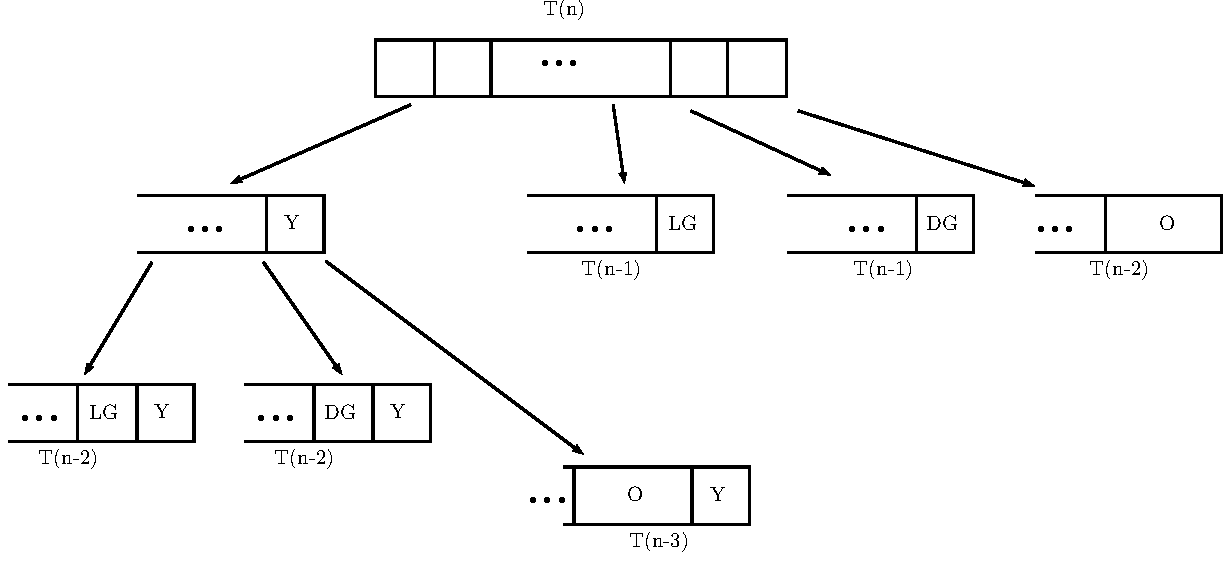
\includegraphics[width=1\linewidth]{tiling}
\end{frame}

\begin{frame}{Quiz 3 Problem 3}
We want to tile the n x 1 strip with 2 x 1 and 1 x 1 tiles, using 2 x 1 tiles of orange color and 1 x 1 tiles of three colors: yellow, light-green and dark green.  Let $T_n$ be the number of such tilings in which no yellow tiles are next to each other.  Determine the fornula for $T_n$ be setting up a recurrence equation...

$$ T_n = 2 \cdot T_{n-1} + 3 \cdot T_{n-2} + 1 \cdot T_{n-3}$$

Initial condition are: \\
    \begin{tabular}{l l l}
        $T_0 = $ & Empty tile & $ = 1$ \\
        $T_1 = $ & Y, LG and DG  & $ = 3$ \\
        $T_2 = $ & O, LG-Y, DG-Y, \dots & $ = 9$ \\
    \end{tabular}
\end{frame}

\section{Red Ridding Hood problem}

\begin{frame}{Red Ridding Hood problem}
    \centering
    \url{http://www.cs.ucr.edu/~acald013/public/tmp/rrh.pdf}
\end{frame}

\end{document}
